\documentclass[aspectratio=169,12pt]{beamer}
\usepackage{amsmath}
\usepackage{amssymb}
\usepackage{xcolor}
\usepackage[most]{tcolorbox}
\usepackage{tikz}
\usepackage{graphicx}
\usepackage[sfdefault,lf]{FiraSans}
\renewcommand{\familydefault}{\sfdefault}
\setlength{\parindent}{0pt}
\everymath{\displaystyle}
\setbeamertemplate{navigation symbols}{}
\setbeamertemplate{footline}{}
\setbeamertemplate{headline}{}
\definecolor{mmpageWhite}{HTML}{FCFBF7}
\definecolor{mmtanSoft}{HTML}{F7F5EF}
\definecolor{mmgreenDeep}{HTML}{244B2C}
\definecolor{mmgreenLeaf}{HTML}{5D8A56}
\definecolor{mmgreenSoft}{HTML}{E4EFD9}
\definecolor{mmtext}{HTML}{163221}
\definecolor{mmanswerColor}{HTML}{306A3A}
\setbeamercolor{background canvas}{bg=mmpageWhite}
\setbeamercolor{normal text}{fg=mmtext,bg=mmpageWhite}
\newtcolorbox{MMCard}[1][]{enhanced,breakable=false,colback=white,colframe=black,boxrule=1.0pt,arc=5pt,left=3pt,right=3pt,top=2pt,bottom=2pt,before skip=0pt,after skip=0pt,height=0.26\textheight,valign=top,#1}
\newcommand{\KoruIcon}{\raisebox{-0.2em}{
\includegraphics[height=1.05em]{img/header-logo.png}}}
\newcommand{\HoeIcon}{\raisebox{-0.2em}{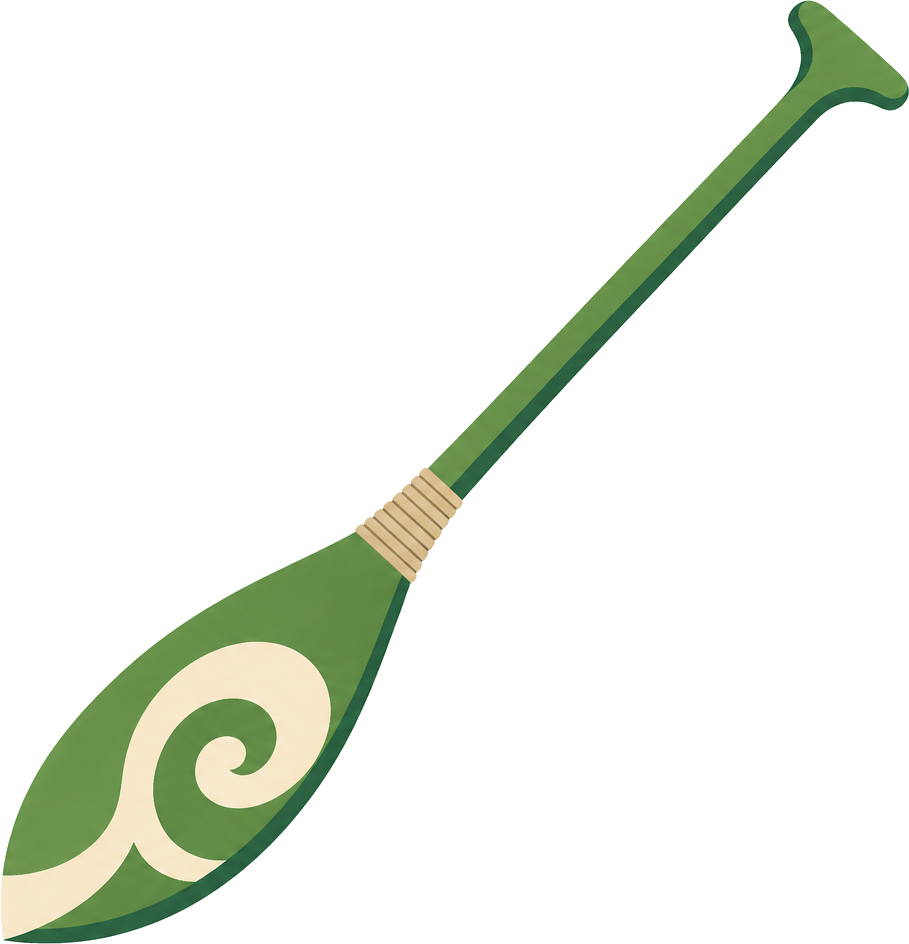
\includegraphics[height=1.05em]{img/hoe.png}}}
\newcommand{\ScaffoldIcons}[1]{\ifcase#1\or \HoeIcon\or \HoeIcon\hspace{0.22em}\HoeIcon\or \HoeIcon\hspace{0.22em}\HoeIcon\hspace{0.22em}\HoeIcon\fi}
\newcommand{\WorksheetTitle}[2]{%
  {\colorbox{mmtanSoft}{\parbox[c][2.0em][c]{0.975\linewidth}{%
    \hspace{0.25em}{\Large\bfseries\textcolor{mmgreenDeep}{#1}\hfill\ScaffoldIcons{#2}}}}
  \par\vspace{0.08em}{\color{mmgreenLeaf}\rule{\linewidth}{2.0pt}}\par\vspace{0.04em}}
}
\newcommand{\MMAnswerTwo}[3]{\begin{MMCard}\raggedright\small\textbf{#1.} \textcolor{mmtext}{#2}\par\vspace{0.1em}\textcolor{mmanswerColor}{\textbf{#3}}\par\end{MMCard}}
\setbeamertemplate{background}{
 \begin{tikzpicture}[remember picture,overlay]
 \draw[black,line width=1.5pt,rounded corners=10pt]
 ([xshift=0.45cm,yshift=-0.45cm]current page.north west)
 rectangle
 ([xshift=-0.45cm,yshift=0.45cm]current page.south east);
 \end{tikzpicture}
}
\begin{document}

\begin{frame}[t]
\WorksheetTitle{Push Tasks — Answers}{3}
\vspace{-0.18em}
\begin{columns}[T,onlytextwidth]
\begin{column}{0.32\textwidth}\MMAnswerTwo{1}{Order 3: angle of rotation?}{120°}\MMAnswerTwo{2}{Order 8: angle of rotation?}{45°}\MMAnswerTwo{3}{60° rotation: order?}{Order 6}\end{column}
\begin{column}{0.32\textwidth}\MMAnswerTwo{4}{120° rotation: order?}{Order 3}\MMAnswerTwo{5}{36° rotation: order?}{Order 10}\MMAnswerTwo{6}{4 lines of symmetry: infer?}{Order is likely 4 (regular)}\end{column}
\begin{column}{0.32\textwidth}\MMAnswerTwo{7}{5 lines of symmetry: infer?}{Order is likely 5 (regular)}\MMAnswerTwo{8}{6 lines of symmetry: infer?}{Order is likely 6 (regular)}\MMAnswerTwo{9}{Relation for regular polygons?}{Lines of symmetry = order of rotational symmetry = n}\end{column}
\end{columns}
\end{frame}

\begin{frame}[t]
\WorksheetTitle{Push Tasks — Answers}{3}
\vspace{-0.18em}
\begin{columns}[T,onlytextwidth]
\begin{column}{0.32\textwidth}\MMAnswerTwo{10}{Order 4, 0 lines: possible?}{Yes — a swastika-like shape}\MMAnswerTwo{11}{Order 2, 0 lines: example?}{A parallelogram}\MMAnswerTwo{12}{Logo with order 3: describe?}{Three-fold symmetric design}\end{column}
\begin{column}{0.32\textwidth}\MMAnswerTwo{13}{Logo with order 6: describe?}{Six-fold symmetric design}\MMAnswerTwo{14}{Dodecagon order 12?}{Yes, regular 12-gon has order 12}\MMAnswerTwo{15}{15-gon: angle of rotation?}{24°}\end{column}
\begin{column}{0.32\textwidth}\MMAnswerTwo{16}{18-gon: angle of rotation?}{20°}\MMAnswerTwo{17}{Formula for angle of rotation?}{360° ÷ n for regular n-gon}\MMAnswerTwo{18}{Matches at 72°,144°,216°,288°: order?}{Order 5}\end{column}
\end{columns}
\end{frame}

\begin{frame}[t]
\WorksheetTitle{Push Tasks — Answers}{3}
\vspace{-0.18em}
\begin{columns}[T,onlytextwidth]
\begin{column}{0.32\textwidth}\MMAnswerTwo{19}{Matches at 40°,80°,120°,160°,200°,240°,280°,320°: order?}{Order 9}\MMAnswerTwo{20}{Matches at 90°,180°,270°: order?}{Order 4}\MMAnswerTwo{21}{Two shapes same order: example?}{Square and rhombus (both order 4 and 2)}\end{column}
\begin{column}{0.32\textwidth}\MMAnswerTwo{22}{Rotational but no reflection: example?}{Parallelogram (order 2, no reflection)}\MMAnswerTwo{23}{Reflection but no rotational: example?}{Isosceles triangle (order 1, 1 line)}\MMAnswerTwo{24}{Traffic sign: order?}{Stop sign: order 8}\end{column}
\begin{column}{0.32\textwidth}\MMAnswerTwo{25}{Car logo: order?}{Mitsubishi: order 3}\MMAnswerTwo{26}{Flag with order 2?}{UK flag: order 2}\MMAnswerTwo{27}{Order > sides: possible?}{No — order can't exceed sides for polygon}\end{column}
\end{columns}
\end{frame}
\end{document}